\documentclass[a4paper]{article}
\usepackage{geometry}
\usepackage{graphicx}
\usepackage{natbib}
\usepackage{amsmath}
\usepackage{amssymb}
\usepackage{amsthm}
\usepackage{paralist}
\usepackage{epstopdf}
\usepackage{tabularx}
\usepackage{longtable}
\usepackage{multirow}
\usepackage{multicol}
\usepackage[hidelinks]{hyperref}
\usepackage{fancyvrb}
\usepackage{algorithm}
\usepackage{algorithmic}
\usepackage{float}
\usepackage{paralist}
\usepackage[svgname]{xcolor}
\usepackage{enumerate}
\usepackage{array}
\usepackage{times}
\usepackage{url}
\usepackage{fancyhdr}
\usepackage{comment}
\usepackage{environ}
\usepackage{times}
\usepackage{textcomp}
\usepackage{caption}
\usepackage{bbm}
\usepackage{enumitem}


\urlstyle{rm}

\setlength\parindent{0pt} % Removes all indentation from paragraphs
\theoremstyle{definition}
\newtheorem{definition}{Definition}[]
\newtheorem{conjecture}{Conjecture}[]
\newtheorem{example}{Example}[]
\newtheorem{theorem}{Theorem}[]
\newtheorem{lemma}{Lemma}
\newtheorem{proposition}{Proposition}
\newtheorem{corollary}{Corollary}

\floatname{algorithm}{Procedure}
\renewcommand{\algorithmicrequire}{\textbf{Input:}}
\renewcommand{\algorithmicensure}{\textbf{Output:}}
\newcommand{\abs}[1]{\lvert#1\rvert}
\newcommand{\norm}[1]{\lVert#1\rVert}
\newcommand{\RR}{\mathbb{R}}
\newcommand{\CC}{\mathbb{C}}
\newcommand{\Nat}{\mathbb{N}}
\newcommand{\br}[1]{\{#1\}}
\DeclareMathOperator*{\argmin}{arg\,min}
\DeclareMathOperator*{\argmax}{arg\,max}
\renewcommand{\qedsymbol}{$\blacksquare$}

\definecolor{dkgreen}{rgb}{0,0.6,0}
\definecolor{gray}{rgb}{0.5,0.5,0.5}
\definecolor{mauve}{rgb}{0.58,0,0.82}

\newcommand{\Var}{\mathrm{Var}}
\newcommand{\Cov}{\mathrm{Cov}}

\newcommand{\vc}[1]{\boldsymbol{#1}}
\newcommand{\xv}{\vc{x}}
\newcommand{\Sigmav}{\vc{\Sigma}}
\newcommand{\alphav}{\vc{\alpha}}
\newcommand{\muv}{\vc{\mu}}

\newcommand{\red}[1]{\textcolor{red}{#1}}
\newcommand{\blue}[1]{\textcolor{blue}{#1}}

\def\x{\mathbf x}
\def\y{\mathbf y}
\def\w{\mathbf w}
\def\v{\mathbf v}
\def\E{\mathbb E}
\def\V{\mathbb V}
\def\ind{\mathbbm 1}

% TO SHOW SOLUTIONS, include following (else comment out):
\newenvironment{soln}{
    \leavevmode\color{blue}\ignorespaces
}{}


\hypersetup{
%    colorlinks,
    linkcolor={red!50!black},
    citecolor={blue!50!black},
    urlcolor={blue!80!black}
}

\geometry{
  top=1in,            % <-- you want to adjust this
  inner=1in,
  outer=1in,
  bottom=1in,
  headheight=3em,       % <-- and this
  headsep=2em,          % <-- and this
  footskip=3em,
}


\pagestyle{fancyplain}
\lhead{\fancyplain{}{Homework 4}}
\rhead{\fancyplain{}{CS 760 Machine Learning}}
\cfoot{\thepage}

\title{\textsc{Homework 4}} % Title

%%% NOTE:  Replace 'NAME HERE' etc., and delete any "\red{}" wrappers (so it won't show up as red)

\author{
\red{$>>$Martin Diges$<<$} \\
\red{$>>$9080689699$<<$}\\
} 

\date{}

\begin{document}

\maketitle 


\textbf{Instructions:} Use this latex file as a template to develop your homework. Submit your homework on time as a single pdf file to Canvas. Late submissions may not be accepted. Please wrap your code and upload to a public GitHub repo, then attach the link below the instructions so that we can access it. You can choose any programming language (i.e. python, R, or MATLAB). Please check Piazza for updates about the homework.
\\\\
\hypersetup{colorlinks=true, linkcolor=cyan}
\url{https://github.com/missingnoglitch0/cs760/tree/main/hw4}

%%% QUESTION 1 %%%


\section{Best Prediction Under 0-1 Loss (10 pts)}
Suppose the world generates a single observation $x \sim \mbox{multinomial}(\theta)$, where the parameter vector $\theta=(\theta_1, \ldots, \theta_k)$ with $\theta_i\ge 0$ and $\sum_{i=1}^k \theta_i=1$.  Note $x \in \{1, \ldots, k\}$.
You know $\theta$ and want to predict $x$. 
Call your prediction $\hat x$.  What is your expected 0-1 loss: 
$$\E[\ind_{\hat x \neq x}]$$
using the following two prediction strategies respectively?  Prove your answer.


Strategy 1: $\hat x \in \argmax_x \theta_x$, the outcome with the highest probability.
\\\\
\textbf{SOLUTION}\\
From the definition of expected value, we have that
$$\E[\ind_{\hat x \neq x}] = 0*P(x = \hat x) + 1*P(x \neq \hat x) = P(x \neq \hat x) = 1 - P(x = \hat x)$$
For a single draw from a multinomial disrtribution, $P(x = j) = \theta_j$. Thus, if we choose the $\hat x$ which satisfies Strategy 1, $$\E[\ind_{\hat x \neq x}] = 1 - \theta_{\hat x}$$

Strategy 2: You mimic the world by generating a prediction $\hat x \sim \mbox{multinomial}(\theta)$.  (Hint: your randomness and the world's randomness are independent)
\\\\
\textbf{SOLUTION}\\
Because our randomness and the world's randomness are independent, the probability that both variables will be observed with some value $j$ is:
$$P(x = j \land \hat x = j) = P(x = j) * P(\hat x = j)$$
Thus, we have that
$$P(x = \hat x) = \sum_{j=1}^{k}{P(x = j \land \hat x = j)} = \sum_{j=1}^{k}{P(x=j) * P(\hat x = j)} = \sum_{j=1}^{k}{\theta_{j}^2}$$

From Strategy 1, we have that $\E[\ind_{\hat x \neq x}] = P(x \neq \hat x) = 1 - P(x = \hat x)$.
Thus, $$\E[\ind_{\hat x \neq x}] = 1 - \sum_{j=1}^{k}{\theta_{j}^2}$$

% Below, for the sake of curiosity,\\
% For $\theta_1 = \theta_2 = .. = \theta_k = \frac{1}{k}$,
% \begin{itemize}
%     \item Strategy 1: $\E[\ind_{\hat x \neq x}] = 1 - 1/k$
%     \item Strategy 2: $\E[\ind_{\hat x \neq x}] = 1 - k(\frac{1}{k})^2 = 1 - 1/k$
% \end{itemize}

% For $\theta_1 = 1, \theta_2 = ... = theta_k = 0$,
% \begin{itemize}
%     \item Strategy 1: $\E[\ind_{\hat x \neq x}] = 1 - 1 = 0$
%     \item Strategy 2: $\E[\ind_{\hat x \neq x}] = 1 - (1)(1) + (k-1)(0)^2 = 1 - 1 = 0$
% \end{itemize}

%%% QUESTION 2 %%%
\newpage

\section{Best Prediction Under Different Misclassification Losses (6 pts)}
Like in the previous question, 
the world generates a single observation $x \sim \mbox{multinomial}(\theta)$.
Let $c_{ij} \ge 0$ denote the loss you incur, if $x=i$ but you predict $\hat x=j$, for $i,j \in \{1, \ldots, k\}$.
$c_{ii}=0$ for all $i$.
This is a way to generalize different costs on false positives vs false negatives from binary classification to multi-class classification.
You want to minimize your expected loss:
$$\E[c_{x \hat x}]$$
Derive your optimal prediction $\hat x$.
\\\\
\textbf{SOLUTION}\\
From the definition of expected value and the knowledge that our randomness and that of the world are independent, we have that 
$$\E[c_{x \hat x}] = \sum_{i=1}^{k}{ \sum_{j=1}^{k}{c_{ij} * P(x=i \land \hat x=j)} } = \sum_{i=1}^{k}{ \sum_{j=1}^{k}{c_{ij} * P(x=i) P(\hat x=j)} } $$
We can extract the probability with respect to $i$ from the inner summation to obtain
$$ \sum_{i=1}^{k}{ P(x=i) \sum_{j=1}^{k}{c_{ij} * P(\hat x=j)} } $$
Given that we are making one optimal prediction $\hat x$, we can fix some $\bar x = \hat x$ which will be our prediction. Thus, $P(\hat x = \bar x) = 1$, $P(\hat x \neq \bar x) = 0$. We can update our expression above to get
$$ \sum_{i=1}^{k}{ P(x=i) \left( c_{i \bar x} * P(\hat x = \bar x) + \sum_{j \in \{ 1, \ldots, k \} / \{\bar x\}}{c_{ij} * P(\hat x=j)} \right) }$$
$$ \sum_{i=1}^{k}{ P(x=i) \left( c_{i \bar x} * 1 + \sum_{j \in \{ 1, \ldots, k \} / \{\bar x\}}{c_{ij} * 0} \right) }$$
$$ \sum_{i=1}^{k}{ P(x=i) \left( c_{i \bar x} \right) }$$
Thus, we will choose an $\bar x = argmin_{\bar x} \sum_{i=1}^{k}{ P(x=i) \left( c_{i \bar x} \right) }$. \\
Expressed verbally, we choose the $\bar x$ which has the lowest sum of $c_{i \bar x}$ over the possible values of $i$, weighting the values of $i$ by their probability of being generated.


%%% QUESTION 3 %%%
\newpage

\section{Language Identification with Naive Bayes (8 pts each)}
Implement a character-based Naive Bayes classifier that classifies a document as English, Spanish, or Japanese - all written with the 26 lower case characters and space.

The dataset is languageID.tgz, unpack it.
This dataset consists of 60 documents in English, Spanish and Japanese. 
The correct class label is the first character of the filename: $y \in \{e, j, s\}$. (Note: here each file is a document in corresponding language, and it is regarded as one data.)

We will be using a character-based multinomial Naïve Bayes model.  You need to view each document as a bag of characters, including space.  We have made sure that there are only 27 different types of printable characters (a to z, and space) -- there may be additional control characters such as new-line, please ignore those.  Your vocabulary will be these 27 character types. (Note: not word types!)


\begin{enumerate}
\item
Use files 0.txt to 9.txt in each language as the training data.
Estimate the prior probabilities 
$\hat p(y=e)$,
$\hat p(y=j)$,
$\hat p(y=s)$
using additive smoothing with parameter $\frac{1}{2}$. 
Give the formula for additive smoothing with parameter $\frac{1}{2}$ in this case. 
Print and include in final report the prior probabilities.
(Hint: Store all probabilities here and below in $\log()$ internally to avoid underflow. This also means you need to do arithmetic in log-space.  But answer questions with probability, not log probability.)

\textbf{SOLUTION}

Additive smoothing: $\hat p (y = l) = \frac{b_l + \alpha}{\sum_{k}{b_k} + \alpha K}$, where $b_l$ is the count for observations of class $l$, $\alpha$ is our smoothing parameter, and $K$ is the number of classes (in this case, the number of languages). Once we make the necessary substitutions, we have
$$\theta_{l} := \hat p (y = l) = \frac{b_l + 0.5}{\sum_{k}{b_k} + 0.5 * 3}$$
After collecting observations and applying smoothing, we have $\hat p(y=e) = \hat p(y=j) = \hat p(y=s) = \frac{1}{3}$


\item
Using the same training data, estimate the class conditional probability (multinomial parameter) for English
$$\theta_{i,e} := \hat p(c_i \mid y=e)$$ 
where $c_i$ is the $i$-th character. That is, $c_1 = a, \ldots, c_{26} = z, c_{27} = space$.
Again use additive smoothing with parameter $\frac{1}{2}$.
Give the formula for additive smoothing with parameter $\frac{1}{2}$ in this case. 
Print $\theta_e$ and include in final report which is a vector with 27 elements.

\textbf{SOLUTION}

$$\theta_{i,e} := \hat p(c_i \mid y=e) = \frac{b_{i,e} + \alpha}{ \sum_{k}{b_{k,e}} + \alpha * K_c }$$
where $K_c$ is the number of character classes $c_1 \ldots c_{27}$, $b_{i,e}$ is the count of occurrences of the character $c_i$ across all documents belonging to language class $e$ (English). As before, $\alpha$ is our smoothing parameter. Once we make the necessary substitutions, we have
$$\theta_{i,e} := \hat p(c_i \mid y=e) = \frac{b_{i,e} + 0.5}{ \sum_{k}{b_{k,e}} + 0.5 * 27 }$$

For $\theta_e$, please see the first column vector in the table below (column e).

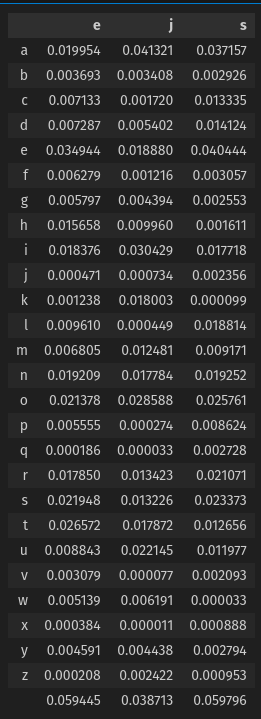
\includegraphics[scale=0.75]{3_2.png}

\item
Print $\theta_j, \theta_s$ and include in final report the class conditional probabilities for Japanese and Spanish.

\textbf{SOLUTION}

Please see the j and s columns in the preceding table for vectors $\theta_j$ and $\theta_s$.

\item
Treat e10.txt as a test document $x$.
Represent $x$ as a bag-of-words count vector (Hint: the vocabulary has size 27).
Print the bag-of-words vector $x$ and include in final report.

\textbf{SOLUTION}

$x = <164, 32, 53, 57, 311, 55, 51, 140, 140, 3, 6, 85, 64, 139, 182, 53, 3, 141, 186, 225, 65, 31, 47, 4, 38, 2, 498>$

Where each entry in the $i$th index of this vector denotes the count of character $c_i$ within document e10.txt

\item
Compute $\hat p(x \mid y)$ for $y=e, j, s$ under the multinomial model assumption, respectively.
Use the formula
$$\hat p(x \mid y) = \prod_{i=1}^d \theta_{i, y}^{x_i}$$
where $x=(x_1, \ldots, x_d)$.
Show the three values: $\hat p(x \mid y=e), \hat p(x \mid y=j), \hat p(x \mid y=s)$.
Hint: you may notice that we omitted the multinomial coefficient.  This is ok for classification because it is a constant w.r.t. $y$.

\textbf{SOLUTION}

We note that $\log{\hat p(x \mid y)} = \sum_{i=1}^d \log{\theta_{i, y}^{x_i}} = \sum_{i=1}^{d}{ x_i \log{\theta_{i, y}}}$

$\hat p(x \mid y=e) = exp(-10904.720647602408)$ \\ 
$\hat p(x \mid y=j) = exp(-11989.469322201065)$ \\
$\hat p(x \mid y=s) = exp(-11338.321401996694)$ \\


\item
Use Bayes rule and your estimated prior and likelihood, compute the posterior $\hat p(y \mid x)$.
Show the three values: $\hat p(y=e \mid x), \hat p(y=j \mid x), \hat p(y=s \mid x)$.
Show the predicted class label of $x$.

\textbf{SOLUTION}

According to Bayes' rule, $\hat p(y \mid x) = \frac{\hat p(x \mid y) p(y)}{p(x)}$. We can express $p(x)$ as $p(x) = \prod_{i=1}^{n}{p(c_i)}$, where $n$ is the number of characters $\in x$ and $p(c_i)$ is the probability of observing a character $c_i$ across all documents. 
It follows that $\log{p(x)} = \sum_{i=1}^{n}{\log(p(c_i))}$.

We can write our first expression in terms of log probabilities:
$$\log{\hat p(y \mid x)} = \log{ \frac{\hat p(x \mid y) p(y)}{p(x)} } = \log{\hat p(x \mid y)} + \log{p(y) - \log{p(x)}}$$

$\hat p(y=e \mid x) = exp(-2904.6029864563616)$\\
$\hat p(y=j \mid x) = exp(-3989.3516610550187)$\\
$\hat p(y=s \mid x) = exp(-3338.2037408506485)$\\

The predicted class label for $x$ will be $e$.

\item
Evaluate the performance of your classifier on the test set (files 10.txt to 19.txt in three languages).
Present the performance using a confusion matrix. A confusion matrix summarizes the types of errors your classifier makes, as shown in the table below.   The columns are the true language a document is in, and the rows are the classified outcome of that document.  The cells are the number of test documents in that situation.  For example, the cell with row = English and column = Spanish contains the number of test documents that are really Spanish, but misclassified as English by your classifier.

\textbf{SOLUTION}

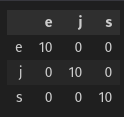
\includegraphics[width=0.2\linewidth]{3_7.png}

\item If you take a test document and arbitrarily shuffle the order of its characters so that the words (and spaces) are scrambled beyond human recognition.  How does this shuffling affect your Naive Bayes classifier's prediction on this document?  Explain the key mathematical step in the Naive Bayes model that justifies your answer.

\textbf{SOLUTION}

Shuffling the order of a test document's characters arbitrarily should not affect the Naive Bayes classifier's prediction. This is because the Naive Bayes model assumes the conditional independence of features. For our model, this means that the probability of one character being present in the input text is assumed to tell us nothing about the probabilities of other characters appearing in the text. In short, the order of characters is not taken into account in our model and thus does not affect its predictions.

\end{enumerate}


%%% QUESTION 4 %%%


\section{Simple Feed-Forward Network (20pts)}
In this exercise, you will derive, implement back-propagation for a simple neural network and compare your output with some standard library’s output. Consider the following 3-layer neural network.

\[
\hat{y} = f(x) = g(W_2\sigma(W_1x))
\]

Suppose $x \in \mathbb{R}^d$, $W_1 \in \mathbb{R}^{d_1 \times d}$, and $W_2 \in \mathbb{R}^{k \times d_1}$ i.e. $f: \mathbb{R}^d \rightarrow \mathbb{R}^k$, Let $\sigma(z) = [\sigma(z_1), ..., \sigma(z_n)]$ for any $z \in \mathbb{R}^n$ where $\sigma(z) = \frac{1}{1 + e^{-z}}$ is the sigmoid (logistic) activation function and $g(z_i) = \frac{exp(z_i)}{\sum_{i=1}^k exp(z_i)}$ is the softmax function. Suppose the true pair is $(x, y)$ where $y \in \{0, 1\}^k$ with exactly one of the entries equal to 1, and you are working with the cross-entropy loss function given below,

\[
L(x, y) = -\sum_{i=1}^k y \text{log}(\hat{y})
\]

\begin{enumerate}
    \item Derive backpropagation updates for the above neural network. (5 pts)
    \item Implement it in NumPy or PyTorch using basic linear algebra operations. (e.g. You are not allowed to use auto-grad, built-in optimizer, model, etc. in this step. You can use library functions for data loading, processing, etc.). Evaluate your implementation on MNIST dataset, report test errors and learning curve. (10 pts)
    \item Implement the same network in PyTorch (or any other framework). You can use all the features of the framework e.g. auto-grad etc. Evaluate it on MNIST dataset, report test errors, and learning curve. (2 pts)
    \item Try different weight initialization a) all weights initialized to 0, and b) initialize the weights randomly between -1 and 1. Report test error and learning curves for both. (You can use either of the implementations) (3 pts)
\end{enumerate}

You should play with different hyperparameters like learning rate, batch size, etc. for your own learning. You only need to report results for any particular setting of hyperparameters. You should mention the values of those along with the results. Use $d_1 = 300$, $d_2 = 200$. For optimization use SGD (Stochastic gradient descent) without momentum, with some batch size say 32, 64, etc. MNIST can be obtained from here (https://pytorch.org/vision/ stable/datasets.html)

\bibliographystyle{apalike}
\end{document}
